%!TEX program=xelatex

\documentclass[a4paper, fontset=none]{article}
\usepackage{ctex}
\usepackage{graphicx}
\usepackage{minted}
\usepackage{amsmath}
\usepackage{hyperref}
\usepackage{wasysym}
\usepackage{geometry}
\geometry{left=2.5cm,right=2.5cm,top=2.5cm,bottom=2.5cm}
\ctexset{fontset=fandol}

\title{信号与系统大作业\\实验报告}
\author{马栩杰\\2014011085\\无43班}
\date{\today}

\begin{document}
\maketitle

华小强手一抖\footnote{``正在他小心翼翼操作的时候,宿舍走廊的装修工地传来了巨大的冲击钻声,他手一抖按下了“乱序并重命名”,所有图像文件被打乱了顺序而且按新顺序改了文件名......''},让上百个电子系同学做了两个多月的大作业... 同学你立功了 \smiley

这次作业主体是用 C++ 来写的,其中用到了 OpenCV 的图片读取、显示、放缩工具和一些矩阵运算的函数。

最开始我用的是 MATLAB ,在 MATLAB 下愉快地完成图像分组以后,我本来准备尝试实现一个看起来很高级的想法\footnote{进行特征点匹配,然后相邻两帧的特征点位移会很小而且其移动应该是明显分组平行的。不过最后我并没有用这种方法来排序..}来进行帧排序,然而尝试调用了图像库中的特征点检测函数以后,我发现这个想法似乎有一点问题:MATLAB 的特征点检测太慢了!找出所有图片的特征点就要用掉将近 5 分钟时间!更不用说再两两做匹配了。此外,由于我对 MATLAB 运行机制不熟悉,如何显式分配内存?数据的生命周期有多长?函数传递参数何时会复制一份数据何时不复制?等等诸如此类的问题导致我在写 MATLAB 代码的时候很不愉快,于是暂且把大作业搁置了起来。

在期末考试结束以后,我学习了一下 OpenCV,在 C++ 中重新实现了一遍前面的内容,然后完成了后面两部分。

虽然用 C++ 来写明显要比 MATLAB 多写很多代码,不过能方便地写面向对象的代码真是太棒了。

\section{图像分组}
\label{sec:图像分组}

最开始我的思路是考虑先手动选取一张演播室的画面,然后计算这个画面与所有画面之间的相似度,相似度超过一个阈值就认为比较的画面是演播室的场景,结果非常轻松就成功了。在分出场景以后我求出了这些画面的平均值,打算用它来作为特征...

\begin{center}
  
\includegraphics[width=0.6\textwidth]{./indoor_average.jpg}
\end{center}

两个主持人的身体几乎没有动,就算是相对比较模糊的脸和手也还是相当清晰的。不过在叠加后的图片里倒是看不出康辉的腮帮子里藏了什么东西\footnote{\url{https://www.zhihu.com/question/34265898}}...

然后我意识到画面里有的地方格外地清晰!对,画面下方 ``中国中央电视台 新闻联播'' 标题所在的位置是固定的。

\begin{center}
  
\includegraphics[width=0.4\textwidth]{./title.jpg}
\end{center}

照常理来考虑,新闻联播的标题位置应该在短期内是不会发生变化的,这就是区分一帧画面是否是室内场景的一个非常好的特征!

\begin{center}
  
\includegraphics[width=0.6\textwidth]{./hehe.jpg}
\end{center}

用这一小块作为特征来做判断非常容易,而且几乎没有出错的可能。


\section{播报画面排序}
\label{sec:播报画面排序}

在分出报道画面之后,就可以对它进行排序啦。

在排序之前,要先做一点准备工作,那就是计算出这些画面两两之间的相似度。为了使计算的时间稍微短一些,首先将图片缩放成 160 $\times$ 120 大小,然后计算两两图片之间的绝对差(用 OpenCV 的 absdiff 函数就可以啦),再将绝对差的各个数位加起来。为了避免重复计算,将计算出的结果存储到一个数组当中,然后需要两个图片相似度的时候直接查表就好咯。

计算完图片之间的相似度,接下来用贪心方法\footnote{为什么是贪心而不是更高级的算法呢?我们面临的问题的一个等价的描述是这样的:已知一个带权无向完全图,求图中的一个最短哈密顿路径。也就是 NP 完全的 TSP 哦.. 个人认为应该可以用一个求 TSP 近似最优解的解法来解决整个问题,然而无情的 ddl 不允许...}产生一个演播室画面的序列。算法大体的流程如下:

\begin{verbatim}
  1 任取一帧画面,放入一个双端队列中
  2 在剩余的画面中分别找到与队列头画面和尾画面相似程度最高的两张图片
  3 如果头画面的相似程度更高,就在队头加入一帧;否则,在队尾加入一帧
  4 回到 2,直到所有画面都已经进入队列
\end{verbatim}

如图所示

\begin{center}
  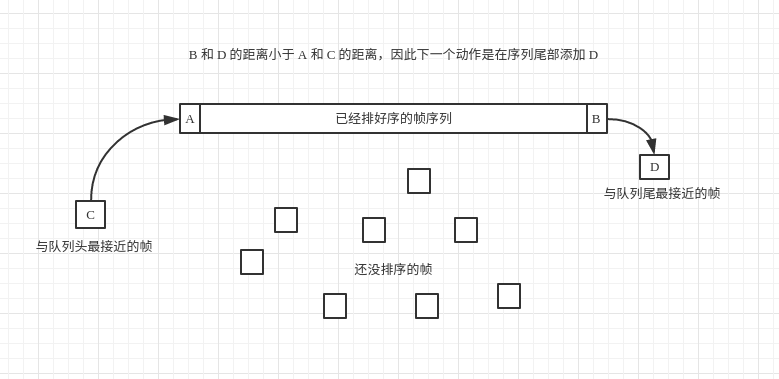
\includegraphics[width=\textwidth]{./sec2.png}
\end{center}

这一算法的实现非常容易。我本来以为单纯用贪心算法并不会得到非常好的结果,然而结果却出乎我的预料,排序以后的画面非常流畅。将排序后的图片序列逐帧播放,画面毫无违和感。

\section{划分镜头与排序}
\label{sec:镜头分组排序}

然后就到了划分镜头的时间啦!

\begin{quotation} \textit{画面左下角有一个小地球不停在转,用小地球的角度就可以标记出每一帧的相位了。} \end{quotation} \begin{flushright} - 谷 GG \end{flushright}

听从谷 GG 的教导,我首先试着提取出画面中的小地球。为了得到一组完整而有序的地球图片,我在网上下载到了一段新闻联播的视频,将视频拆分为每秒 25 帧的图片序列,然后再取出其左下角的一小块。

但是并不知道小地球旋转的周期是多少?只要随便取地球的一个相位然后和所有画面中的地球依次比对就好了。如果用地球做相位的想法可靠的话,那么绘出表示它们相似性曲线一定会有很明显的周期性。

\begin{center}
  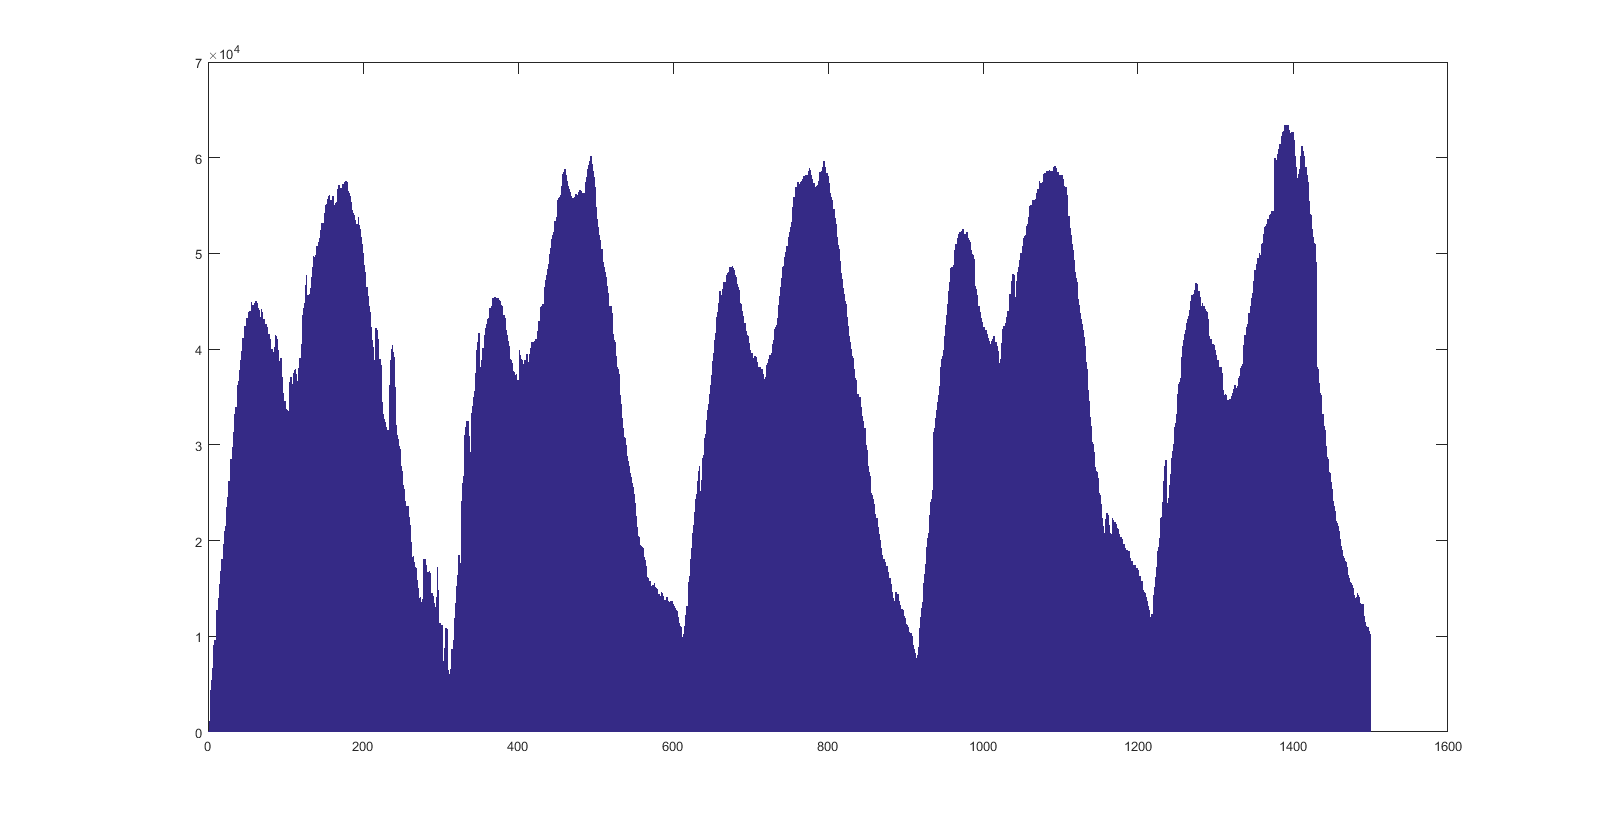
\includegraphics[width=\textwidth]{./earth.png}
\end{center}

果然,小地球区域的绝对差有明确的周期。经过计算得知这一周期是 302 帧\footnote{为什么不是 300 呢?这不科学..} 。

于是只要截取下来这些地球的画面就可以确定出每一帧的相位了。

\begin{center}
  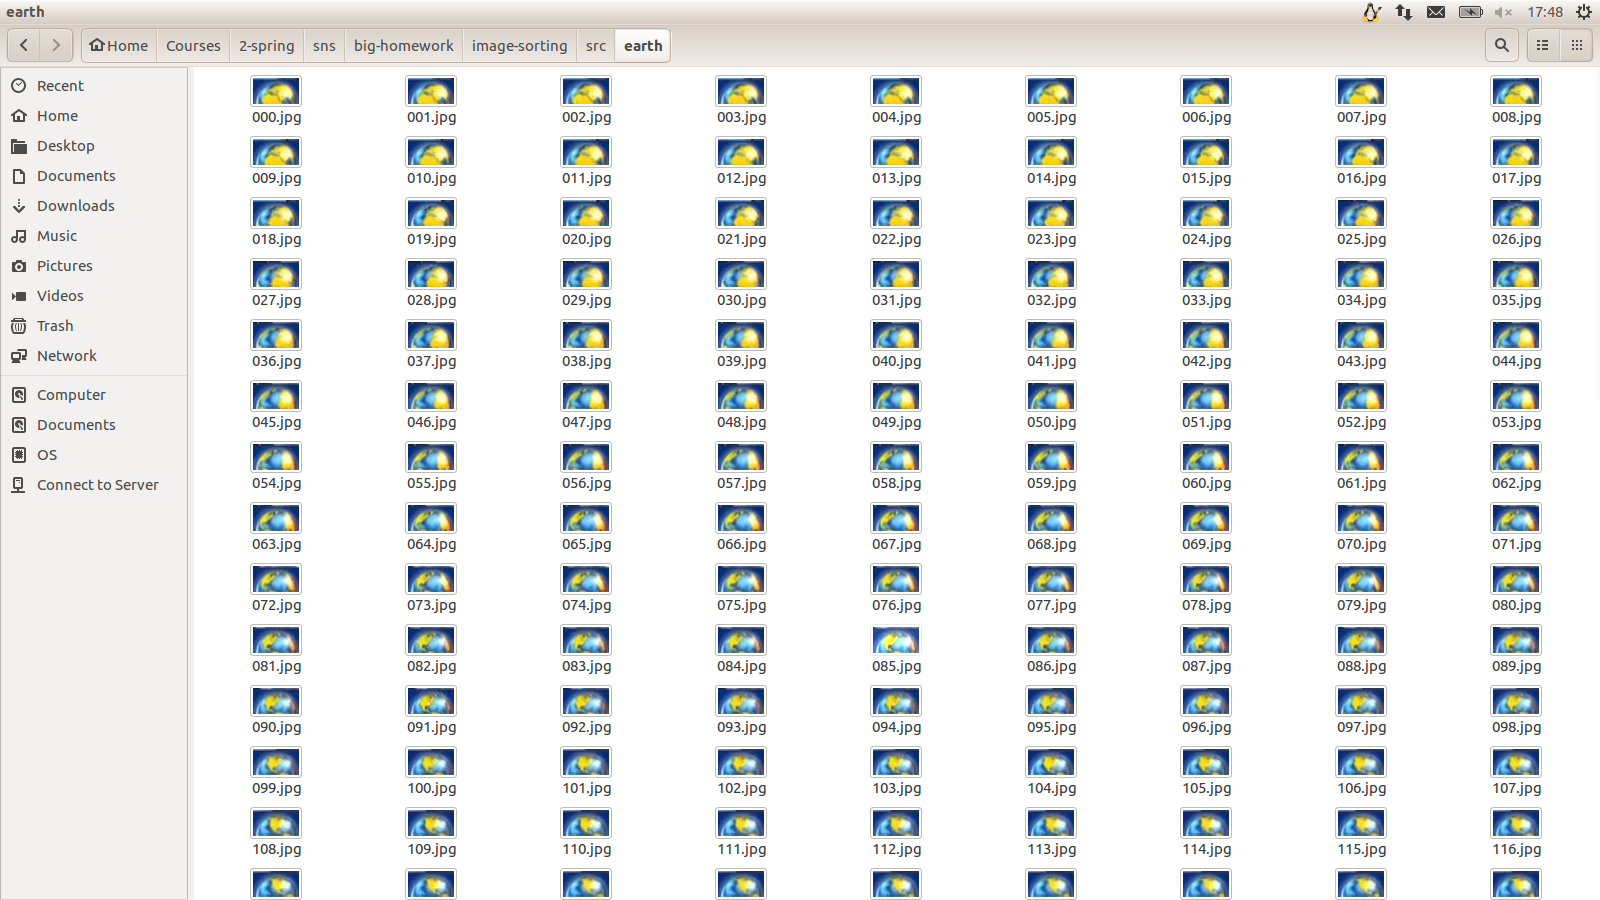
\includegraphics[width=\textwidth]{./many_earth.png}
\end{center}

确定出相位有什么用呢?我陷入了沉思..

总会有用的!先把相位放在一边,试着划分镜头吧。

一个很容易想到的办法是根据图像的内容对图片进行聚类。然而,在实际操作过程中,我发现用聚类方法划分镜头很难做。首先,类的数量无法预先确定。如果不能提前确定类数量的话,就需要在一次聚类后对聚类的结果进行分析,然后手动合并拆分一些类,或者尝试改变参数再聚类。其次,在实际操作的过程中,经常会出现几个不同的镜头被放进了一个类中,或者一个镜头的画面被放进多个不同类的情况。而且在聚类以后再进行贪心排序也会因为类中的图像可能并不完整而导致排序后的结果非常糟糕。

在不断摸索的过程中,我想到了另外一种做法。

首先,尝试用贪心方法对所有帧排序。由于同一个镜头内部相邻的两帧之间的相似程度很高,所以贪心排序会使得相邻帧有很大概率被排成有序的序列。经过这次排序以后,可以产生一个帧序列,这个序列是分段连续的。这里所说的分段连续指的是大约每几十帧画面是连续的一段内容,然后由于各种原因有一定概率某一帧接下来会匹配到一个跟这一帧相似度不是很高的画面(但依然是剩下的所有画面中与该帧匹配度最高的一帧),然后贪心匹配会在新的一帧的基础上继续进行,于是我们就可以得到一个分段连续的帧序列。

接下来要做的事情是把帧序列中连续的块分割出来。在代码实现中,对分段连续帧序列顺序扫描,如果接下来的一帧与前一帧之间的绝对差小于一个阈值(用当前镜头所有相邻帧两两之间的绝对差的平均值来确定),则接下来的一帧与前一帧在同一镜头当中,并且认为这两帧是连续的。而如果绝对差大于阈值,则认为接下来的一帧在一个新的镜头中。

经过这样的拆分操作之后,原始的无序图片被划分为几百个块(Scene)。相比最初的 3000 多帧画面,这已经是一个相当大的前进了。此时,可以根据每一帧的相位信息确定这个块的帧序列是顺序还是逆序的,并且将逆序的块翻转,为接下来的处理做铺垫。这时的帧块就像是一堆乐高积木一样,每个块内部都是连续的,但是块与块之间还可能能拼合为更大的块。在接下来的处理过程中,帧块就是进行处理的基本单位。

虽然现在已经将所有画面成功分割成了几百个分段连续的块,但是这些块并不都是独立的镜头。由于最开始采用了贪心方法这种简单的方法对帧进行匹配,一定会有同一个镜头的画面被放在几个不同的块中的情况出现。为了将这些本来应该在一起的块拼合起来,接下来同时考虑两个块首尾的相似度和相位信息对块进行拼接。判断所有块两两头尾之间的相位差,如果有两个块的头尾相位是连续的,那么接下来判断头尾间的绝对差,如果绝对差小于一个阈值(根据两个镜头内相邻帧绝对差的平均值来确定),那么就认为这两个块应该是在同一个镜头内相邻的。这里所做的事情也可以理解为以块为单位做贪心匹配,只不过在贪心匹配中的距离函数加入了绝对差阈值和相位的约束。

通过逐步调整阈值,经过几次块拼接以后,数百个块就被拼成了相位连续的几十个块,也就是最终划分出的几十个镜头。

最后,两两镜头之间的画面差异都很大,只需要根据相位信息再次用贪心方法\footnote{好像整篇文章都是贪心 orz}将所有镜头排序就好了!

总的来说最后排好序的视频还是基本能看的,与使用聚类方法做的结果相比,画面鬼畜的情况要少很多,只不过在播放中偶尔会出现一闪而过的零碎片段。由于有这些没有被正确分组的片段的存在,因此最终镜头间排序的效果并不好。

不过由于没有使用更复杂的算法,程序的运行速度很快,大概 3 分钟以内就可以跑完\footnote{Intel i5 4核,8G DDL3 低压内存,机械硬盘}。

\section{前景展望}
\label{sec:前景展望}

在此结果的基础上,我认为如果采用先进行聚类,大致划分一下镜头,然后再对每个镜头用 TSP 近似解算法排序、分块,然后将所有分好的块放在一起再进行拼接,可以解决出现零碎块的问题,或许会得到更好的结果,而且也可以更加充分地利用 10 min 的运行时间\footnote{然而 ddl 不允许,而且大作业只有 5 分..}。

\section*{附录A 程序运行方式}
\label{sec:程序运行方式}

这次大作业是用 C++ OpenCV 写的,我在 Ubuntu 下配置了 OpenCV 的环境,所有代码都是在 Linux 中完成的,因此也只编译了在 64 位 Linux 下运行的版本。

使用方式:

\begin{verbatim}
      image-sorting [IMAGE_DIRECTORY]
\end{verbatim}

在命令行下向 image-sorting 程序输入图片所在的文件夹的地址就好啦!

然后程序就会开始运行,在运行过程中会有一些人性化的提示,说明程序当前运行到了什么地方。在结束运算以后,程序会将结果输出到几个 txt 文件中,并且会询问是否需要播放已经排好序的视频(默认是不播放)。

需要注意的是程序在运行中要读取此前处理好的演播室画面下的标题和外景的小地球,因此可能需要避免移动 image-sorting 的位置以防止它找不到这些数据。

为了避免出现问题,也可以考虑直接修改 code 文件夹中的 run.sh 文件,在对应的位置填写好图片文件夹的路径然后直接运行 run.sh 就可以啦。

如果出现各种问题运行不了程序的话请联系我。

\section*{附录B 编译环境配置}
\label{sec:编译环境配置}

虽然我写了自动化构建和编译项目的 script,然而如果想编译一下整个程序的话,首先需要在 Linux\footnote{在 ListDir 函数中用到了 Posix 接口,如果一定要在 Windows 下编译的话请联系我改代码。} 下安装 OpenCV(3.1.0)、 CMake 以及 Make。

安装 Make 和 CMake(Ubuntu: \mintinline{bash}{sudo apt-get install make cmake}),然后根据 OpenCV 的文档编译安装 OpenCV (\url{http://docs.opencv.org/3.1.0/d7/d9f/tutorial_linux_install.html},需要解决一些依赖问题,注意在下载的时候要选择 3.1.0),在编译成功 OpenCV 以后,首先删除 code 文件夹中的 release 文件夹,然后依次执行 cmake-build.sh 和 build.sh,就可以在 release 文件夹中找到编译好的 image-sorting 了。

\section*{附录C 使用工具}
\label{sec:使用工具}

\paragraph{MATLAB}
\label{par:MATLAB}
新闻联播标题提取、小地球提取、小地球相位分析。

\paragraph{OpenCV}
\label{par:OpenCV}
C++ 中读取与显示图片、对图片进行矩阵运算。
\footnote{\url{http://opencv.org/}}

\paragraph{GNU Make}
\label{par:GNU Make}
\footnote{\url{https://www.gnu.org/software/make/}}

\paragraph{CMake}
\label{par:CMake}
\footnote{\url{https://cmake.org/}}

\paragraph{you-get}
\label{par:you-get}
一个开源的命令行网页视频下载工具,用来下载新闻联播视频。
\footnote{\url{https://github.com/soimort/you-get}}

\paragraph{ffmpeg}
\label{par:ffmpeg}
著名的 GNU 命令行视频解码软件,用来将下载到的视频拆分为帧序列。
\footnote{\url{https://ffmpeg.org/}}

\paragraph{ProcessOn}
\label{par:ProcessOn}
绘制贪心算法描述图用到了这个在线绘图工具。
\footnote{\url{https://www.processon.com/}}

\end{document}
